\chapter{The Arithmetic of Durable Wealth}

This lecture gives us no blackboard and no formal theorem, yet it carries a surprisingly clean mathematical spine. We are first shown scale, then leverage, then cash flow, then operational measurement, then survival under volatility. The order matters. We do not begin with doctrine. We begin with the feeling of magnitude, and only after that do we ask what mechanisms separate large wealth from ordinary earnings. If we read the lecture carefully, the moving parts are fairly crisp: debt raises fragility, retained cash compounds into assets, measured operations can be copied, cheaper locations can be made to behave like better ones, and unstable income requires reserves.

\section{Scale First, Explanation Second}

The lecture opens by making size visible before it explains anything. We are handed Ramsey's annual business revenue, Ramsey's real-estate magnitude, Jimmy John's exit value, and Charlie Sheen's celebrity-income aura. This is not yet the blueprint. It is the condition under which the audience will take the blueprint seriously.

The cleanest numerical markers in the opening are
\begin{align}
R_{\mathrm{Ramsey}} &\approx \$300 \times 10^6/\text{yr},\\
V_{\mathrm{campus}} &\approx \$650 \times 10^6,\\
V_{\mathrm{RE}} &\approx \$850 \times 10^6,\\
V_{\mathrm{Jimmy}} &\approx \$3.5 \times 10^9.
\end{align}
These quantities are not all the same kind of thing. One is annual business revenue, two are real-estate valuations, and one is a company-sale valuation. The lecture's first task is therefore not to give us a theorem, but to force us to separate gross flow from owned stock and business income from sale value.

Charlie Sheen is introduced differently. There the lecture gives prestige and public scale rather than a precise balance-sheet quantity. That is already instructive. Sometimes wealth is framed through hard numbers; sometimes it is framed through cultural position and the memory of very large paychecks. The lecture will later use Charlie as a different kind of case: not enterprise buildout, but survival when the income spigot can narrow or shut off.

\section{Debt, Fragility, and the Ramsey Refusal}

Ramsey's first mathematically serious point is stated in ordinary speech:
\begin{equation}
\text{Debt} = \text{risk}.
\end{equation}
Taken literally, that sentence is too compressed. Taken structurally, it is the kernel of an anti-leverage model. Let \(D\) denote debt, \(DS\) the associated debt service, and \(F\) the fragility of the enterprise under revenue interruption. Then the lecture's logic can be rendered as
\begin{equation}
\frac{\partial F}{\partial D} > 0,
\end{equation}
and more concretely as
\begin{equation}
DS>0 \ \land\ R_t\downarrow \ \Rightarrow\ P(\text{distress})\uparrow.
\end{equation}
The point is not that every dollar of debt instantly produces failure. The point is that debt creates a fixed claim, and fixed claims become most dangerous when revenue becomes uncertain.

\paragraph{Anecdote.} The host presses the obvious objection: even the biggest companies borrow. Why refuse the extra capital if it would seem to increase the speed of scaling?

\paragraph{Claim.} Ramsey's claim is that he does not borrow money at all, ever, for anything.

\paragraph{Mechanism.} Slow organic growth is accepted as the price of lower fragility. The COVID example functions as the stress test. If the business has no debt service, revenue interruption need not mechanically force insolvency.

\subsection{Question \& Answer}

\paragraph{Question.} If major firms borrow to scale, why refuse debt entirely?

\paragraph{Answer.} Because the lecture's standard of success is not simply top-line speed; it is survival under stress. Debt finances speed by creating a fixed claim. If revenue later falls, the claim does not fall with it. Ramsey therefore accepts slower growth in exchange for a lower probability that a shock turns into a business-ending event. In symbolic form, his working intuition is
\begin{equation}
DS=0 \ \Rightarrow\ P(\text{insolvency}\mid R_t\downarrow)\ \text{is reduced}.
\end{equation}
This is not a complete balance-sheet theorem. It is a clear operating rule.

\section{Buying Dirt First}

Once the lecture states its anti-debt principle, it immediately raises the harder question: how does one then buy large property? Ramsey's answer is practical rather than mystical. Buy the land first, build later, and let operating cash do the work.

The first transaction is given with unusual precision:
\begin{equation}
P_0=\$10 \times 10^6,\qquad A_0=48\ \text{acres}.
\end{equation}
The key detail is not only price or acreage. The key detail is that the land is acquired before the cash exists to develop it fully. ``We just bought the dirt'' is therefore one of the lecture's strongest lines. The object is controlled first; the full buildout is deferred.

The capital loop behind this can be written cautiously as
\begin{equation}
K_{t+1}=K_t+CF_t-C_{\mathrm{draw},t}-I_t,
\end{equation}
where \(K_t\) is retained capital, \(CF_t\) is operating cash flow, \(C_{\mathrm{draw},t}\) is cash removed for spending or owner draw, and \(I_t\) is reinvestment into land or buildings. The lecture's phrase ``we just kept dumping everything we made into this concrete thing here'' licenses exactly this type of recurrence.

\begin{figure}[h]
\centering
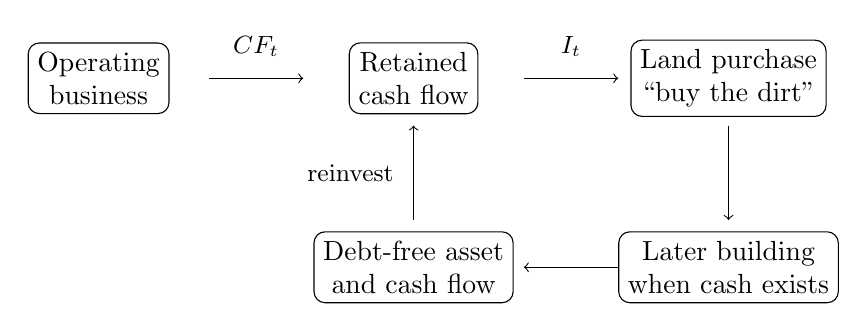
\begin{tikzpicture}[scale=1]
\node[draw, rounded corners, align=center] (op) at (0,0) {Operating\\business};
\node[draw, rounded corners, align=center] (cf) at (4,0) {Retained\\cash flow};
\node[draw, rounded corners, align=center] (land) at (8,0) {Land purchase\\``buy the dirt''};
\node[draw, rounded corners, align=center] (build) at (8,-2.4) {Later building\\when cash exists};
\node[draw, rounded corners, align=center] (asset) at (4,-2.4) {Debt-free asset\\and cash flow};

\draw[->] (1.4,0) -- (2.6,0);
\draw[->] (5.4,0) -- (6.6,0);
\draw[->] (8,-0.6) -- (8,-1.8);
\draw[->] (6.6,-2.4) -- (5.4,-2.4);
\draw[->] (4,-1.8) -- (4,-0.6);
\node at (2,0.4) {\small \(CF_t\)};
\node at (6,0.4) {\small \(I_t\)};
\node at (3.2,-1.2) {\small reinvest};
\end{tikzpicture}
\caption{Transcript-based reconstruction of Ramsey's cash-funded real-estate loop.}
\end{figure}

\paragraph{Worked Example.} The 2008 dislocation gives the lecture a simple arithmetic example. Ramsey says he bought assets at roughly \(15\%\) to \(20\%\) of former price. If a property had once traded at
\[
P_{\mathrm{former}}=\$10 \times 10^6,
\]
then the crisis purchase range would be
\begin{align}
P_{\mathrm{buy,low}} &\approx 0.15\,P_{\mathrm{former}}=\$1.5 \times 10^6,\\
P_{\mathrm{buy,high}} &\approx 0.20\,P_{\mathrm{former}}=\$2.0 \times 10^6.
\end{align}
The lecture is not claiming every former \$10 million property became purchasable for \$1.5--\$2.0 million. It is showing what cash plus patience can do when the market reprices violently.

\subsection{Question \& Answer}

\paragraph{Question.} How do we buy large real estate without borrowing?

\paragraph{Answer.} The lecture's answer comes in stages. First control land, even if the full development must wait. Then let the operating business generate cash. Then retain rather than extract that cash. Then build when the retained stock is large enough. Finally, when crisis discounts appear, use cash to convert patience into acquisition power. The logic is sequential, not magical.

We can also formalize Ramsey's ``positive snowball'' in a clean way. Suppose debt-free properties \(1,\dots,n\) throw off cash flows \(CF^{(1)},\dots,CF^{(n)}\), and let \(E_{n+1}\) be the equity needed for the next property. Then the next acquisition becomes feasible once
\begin{equation}
\sum_{i=1}^{n}\sum_{t=0}^{T-1} CF_t^{(i)} \ge E_{n+1}.
\end{equation}
That is precisely why Ramsey says the first one is hardest, then the second, then the third. The snowball exists, but only after the early base is built.

\section{No Rescuer, No Easy Button}

The Ramsey interview does not remain inside finance. It widens into a general theory of progress. Nobody is coming to save us. Nobody is coming to discover us. The lecture converts this into a repeated-action model: get up, leave the cave, do the work, and then do it again tomorrow.

A clean way to render that cumulative idea is
\begin{equation}
X_N = X_0 + \sum_{t=0}^{N-1}\delta_t,
\end{equation}
where no single \(\delta_t\) has to be dramatic. This is our careful mathematical version of ``one tiny little step at a time'' and ``one tiny conversation at a time.'' The lecture's point is that large visible outcomes are often the integrated effect of many small increments.

The generational discussion then shifts the frame once more. Technology has made many things feel instantaneous, and the lecture argues that this breeds a search for an easy button. The tension is not between young and old as such. It is between immediacy and patience. Ramsey's last version of the same idea is culinary: the best barbecue is cooked slowly, not microwaved.

A brief but revealing modern detour follows. The host compresses Ramsey's lesson into the phrase that billionaires ``get their money to work for them while they sleep,'' then immediately sells access to a live investing event. We should not let that detour dominate the chapter, but we should notice what it does. Interpretation itself has become a product. Billionaire doctrine is not only reported; it is packaged.

\section{Measurement, One-Page Assets, and the Jockey}

Jimmy John's interview changes the texture of the lecture. Ramsey speaks like a conservative allocator who distrusts leverage. Jimmy speaks like an operator who learned how to copy a machine.

The crucial origin point is dated and counted:
\begin{equation}
N_{\mathrm{sub},1987}=4,\qquad N_{\mathrm{PizzaHut,mentor}}=25.
\end{equation}
Jamie Coulter's lesson is then given in its most compressed form:
\begin{equation}
x\ \text{unmeasured} \Rightarrow x\ \text{unmanaged}.
\end{equation}
Again, this is not a theorem in the hard mathematical sense. It is an operating identity. If the variable is not tracked, disciplined control is impossible. And if disciplined control is impossible, copyable scale is weak.

\paragraph{Anecdote.} The mentor already has 25 Pizza Huts, has built and sold chains, and shares process. Jimmy is still small enough that this advice can rewire the business rather than merely decorate it.

\paragraph{Claim.} ``If you can't measure it, you can't manage it.''

\paragraph{Mechanism.} Known numbers support repeatable procedure. Repeatable procedure supports multi-store scale.

Jimmy then gives a second filter, this time for investing rather than store management. He says he only does things he understands, and he wants to be able to understand them on a single sheet of paper. We can encode that filter as
\begin{equation}
I(a)=1 \iff a\ \text{can be understood on one sheet and related to concretely}.
\end{equation}
Land and farm ground pass this test for him. Opaque stories do not.

The farm-ground cycle is almost embarrassingly simple:
\begin{equation}
\text{land}+\text{inputs}\rightarrow \text{plant}\rightarrow \text{rain risk}\rightarrow \text{harvest}\rightarrow \text{sale}.
\end{equation}
That simplicity is precisely the point. The lecture is not hunting novelty. It is hunting intelligibility.

Jimmy's third investing rule is person-centered:
\begin{equation}
E[R\mid q_{\mathrm{operator}}] > E[R\mid \text{asset story alone}].
\end{equation}
He calls this ``bet the jockey, not the horse.'' One need not pretend the inequality is formally estimated. It is enough to notice the ordering of priorities: operator quality first, asset romance second.

\subsection{Question \& Answer}

\paragraph{Question.} What should we buy if we do not yet know how to invest?

\paragraph{Answer.} Jimmy's answer is not ``buy what is fashionable.'' It is ``buy what you can actually understand.'' If the asset is simple enough to fit on one page, relatable enough to be pictured concretely, and controlled by a person who performs rather than tells stories, then the allocation passes the filter. Land, farmland, and operator-backed deals are his favored cases precisely because their mechanics stay legible.

\section{Turnarounds, Reverse Pitch, and B/C Rent into A Sales}

The Jimmy interview becomes still more technical when the host goes back to 2003 and the failing-store problem:
\begin{equation}
N_{\mathrm{stores}}\approx 200,\qquad N_{\mathrm{failing}}\approx 70.
\end{equation}
The natural expectation is that the fix will be some clever financial engineering. Instead Jimmy says the first change was that he quit selling and started telling the truth. The sandwich business is 24-7, 365. It is a lifestyle. It is a grind. Franchises were then sold one at a time, not in large protected territories.

The lecture is making a hard claim here. Better growth came from stricter selection and truer signaling rather than from more aggressive persuasion. This ``reverse pitch'' is one of the most interesting mechanisms in the episode. By telling people not to do it unless they were truly ready, Jimmy got better operators.

The later outcome is given in long-horizon form:
\begin{equation}
N_{\mathrm{later}}\approx 2500.
\end{equation}
That is not credited to one trick. It is credited to a more disciplined operator-selection machine.

The final Jimmy mechanism is delivery. Prime A locations were too expensive. So cheaper B and C locations were taken instead, and delivery plus relentless sampling was used to widen the demand radius. The lecture's cleanest business equation is therefore
\begin{equation}
r_{BC}+h_{\mathrm{delivery}} \Rightarrow Q_A,
\end{equation}
where \(r_{BC}\) is lower rent from weaker locations, \(h_{\mathrm{delivery}}\) is delivery hustle plus off-site sampling, and \(Q_A\) is A-level sales. In words: B/C rent can be combined with delivery and field marketing to produce the sales quality of a better location.

\begin{figure}[h]
\centering
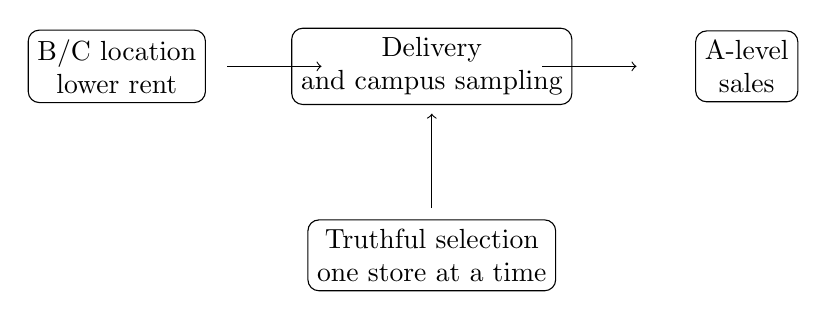
\begin{tikzpicture}[scale=1]
\node[draw, rounded corners, align=center] (rent) at (0,0) {B/C location\\lower rent};
\node[draw, rounded corners, align=center] (delivery) at (4,0) {Delivery\\and campus sampling};
\node[draw, rounded corners, align=center] (sales) at (8,0) {A-level\\sales};

\draw[->] (1.4,0) -- (2.6,0);
\draw[->] (5.4,0) -- (6.6,0);

\node[draw, rounded corners, align=center] (discipline) at (4,-2.4) {Truthful selection\\one store at a time};
\draw[->] (4,-1.8) -- (4,-0.6);
\end{tikzpicture}
\caption{Transcript-based reconstruction of Jimmy John's location arbitrage and franchise-discipline model.}
\end{figure}

\subsection{Question \& Answer}

\paragraph{Question.} What actually fixed the failing stores, and why did delivery become such a decisive edge?

\paragraph{Answer.} The stores were not saved by glamour or by a softer sales pitch. They were stabilized by changing the quality of the operator pool and by telling the truth about the grind. Delivery then solved a different problem. It allowed cheaper real estate to behave like better real estate by shifting demand generation out into the field. The lecture's deeper point is that competitive advantage often comes from altering the geometry of the business rather than merely polishing the product.

\section{Rainy Days, Rainy Decades}

Charlie Sheen is used differently from Ramsey and Jimmy. He is not primarily a case of enterprise compounding. He is a case of unstable high-income life. That is why his main mathematical contribution is reserve logic.

His advice can be written in the plainest possible update rule:
\begin{equation}
S_{t+1}=S_t+Y_t-C_t,
\end{equation}
where \(S_t\) is reserve savings, \(Y_t\) is income inflow, and \(C_t\) is spending. The lecture's warning is that one must never assume the spigot stays open. A rainy day can become a rainy decade. In other words,
\begin{equation}
Y_t \not\equiv \text{constant} \Rightarrow S_t\ \text{must buffer a multi-period drought}.
\end{equation}
This is not subtle mathematics, but it is serious mathematics. Volatile income requires stored slack.

The second Charlie principle is not financial but existential. Hollywood may put the person in timeout. That does not automatically put the mind in timeout. The lecture's compressed identity is
\begin{equation}
\text{industry timeout} \neq \text{self-timeout}.
\end{equation}
He then moves toward a more general ethic: believe in yourself when others do not, accept that people will surprise you, do not let the collapse of reputation become the collapse of agency, and honor the work no matter what.

\paragraph{Anecdote.} The host explicitly frames Charlie as a man of extreme public highs and lows.

\paragraph{Claim.} It is never too late to get a fresh start.

\paragraph{Mechanism.} The fresh start becomes possible if reserves exist, if the self does not collapse when the institution turns away, and if the discipline of work survives the reputational event.

\subsection{Question \& Answer}

\paragraph{Question.} What do we do when the spigot shuts off?

\paragraph{Answer.} Save before it shuts off. That is the first answer. The second is psychological rather than financial: do not grant the external world the authority to shut down the inward engine. Charlie's section is the lecture's coda on volatility. Ramsey teaches us how not to become fragile by leverage. Charlie teaches us how not to become fragile by assuming today's income lasts forever.

\section{Summary}

The lecture begins with spectacle and ends with discipline. Ramsey gives us the anti-debt and cash-funded real-estate model:
\[
\text{less leverage} \Rightarrow \text{less fragility}, \qquad
\text{retained cash} \Rightarrow \text{owned assets}.
\]
Jimmy John gives us the operator's model:
\[
\text{measure} \Rightarrow \text{manage}, \qquad
\text{understand} \Rightarrow \text{invest}, \qquad
\text{deliver} \Rightarrow \text{turn weak location into strong sales}.
\]
Charlie then gives us the volatility model:
\[
\text{save against drought}, \qquad
\text{do not let public collapse become inward collapse}.
\]

What the lecture finally offers is not one secret. It offers a small family of recursions. Retain rather than borrow. Reinvest rather than display. Measure rather than improvise. Select operators rather than chase stories. Save as if the spigot can close. And do the small thing again tomorrow.